Para el análisis de los resultados generamos 10 ejecuciones 
en la sección \textit{Desarrollo}.
Luego, generamos dos gráficos para analizar los resultados de los experimentos.
Categorizamos los valores de cada celda dependiendo su rango en partido
\textit{A, B o I }. Para A, si se encuentra en el rango [-3, -1], Indeciso [-1, 1]  y B si se encuentra en el rango [1, 3].

La figura \ref{fig:modelo_shock_box} describe la cantidad de celdas finales que
finalizaron la simulación siendo del partido \textit{A, B o I (indeciso)}.

Cada sub-gráfico corresponde a uno de los experimentos detallados. En el eje de
las X se encuentra cada estado final que pudo haber alcanzado una celda. En el
eje de las Y tenemos el conteo correspondiente.  Cada punto de cada columna
corresponde a una ejecución de cada experimento con lo cual por cada
sub-gráfico se encuentran 10 mediciones con el resultado de cada ejecución.


En el caso de \textit{Shocker 0} se puede observar que el estado inicial de las
celdas determina el estado final de estas dado que no se observan shocks
externos. Esto significa que su estado está dado únicamente por la dinámica de
interacción entre las celdas.

Decidimos tomar este estado inicial de las celdas para, luego de estimularlas
con los shocks, analizar si era visible la dinámica generada por estos.
Este caso, nos da un \textit{baseline} contra el cual poder razonar.

En el caso de Shockers balanceados (misma cantidad de Shockers de tipo A  y de
B) que se observa en \textit{2A 1I 2B} el Shocker
pareciera aumentar la varianza muestral de los datos finales con respecto al
caso que no presenta estímulos exógenos.

Es muy distinto el caso de Shockers balanceados en el cual los Shockers que generan
Indecisos tiene más de un 50\% de participación, el gráfico \textit{1A 3I 1B}.
En este caso se observa que los indecisos tienen mucha influencia y que estos
mantienen su estado al finalizar la simulación aun siendo que inicialmente eran una minoría.
Los Shockers de indecisos en este caso sirven como un neutralizador de opiniones.

Es importante notar cómo cambia el comportamiento entre los casos \textit{2A 1I 2B} y \textit{2A 2I 1B}. Se observa que al aumentar la cantidad de Shocks de indecisión el más influyente (A) toma partido de ello y copta la mayor parte de la población.



\begin{figure}[!h]
\centering
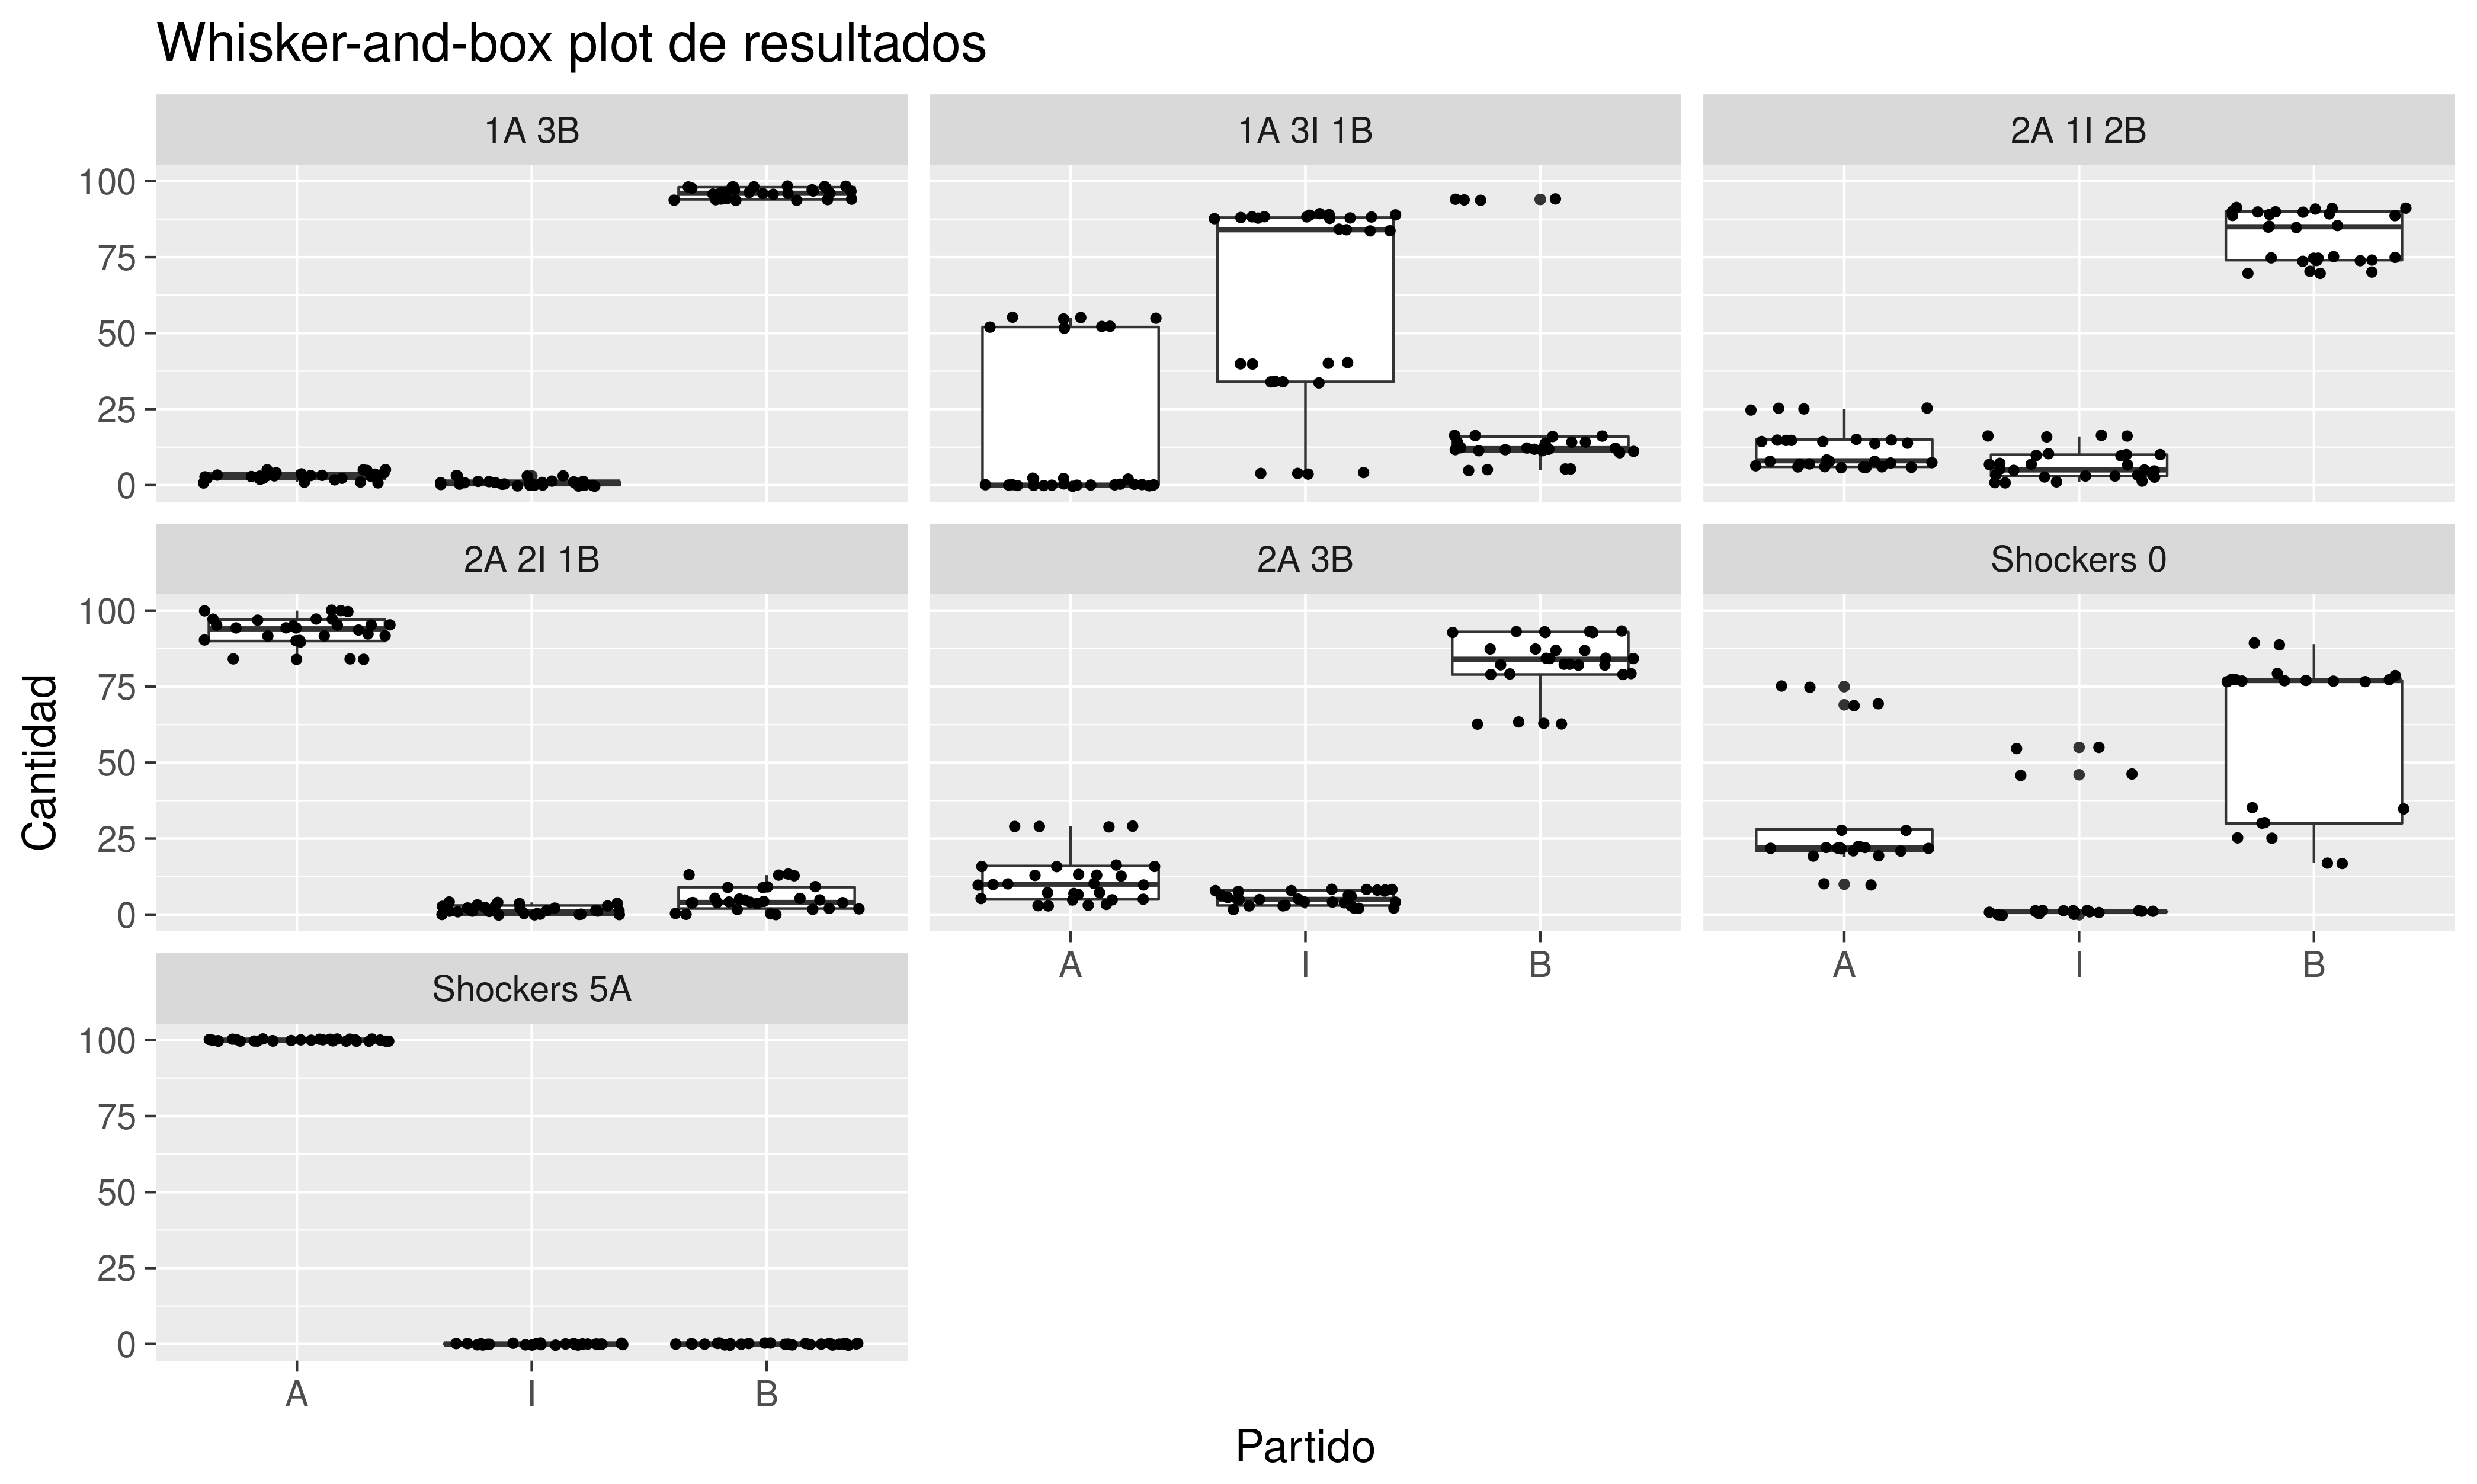
\includegraphics[scale=0.5]{imagenes/histograma_resultados.png}
    \caption{\textit{Whisker-and-box} plot para los resultados del modelo}
\label{fig:modelo_shock_box}
\end{figure}

\begin{figure}[!h]
\centering
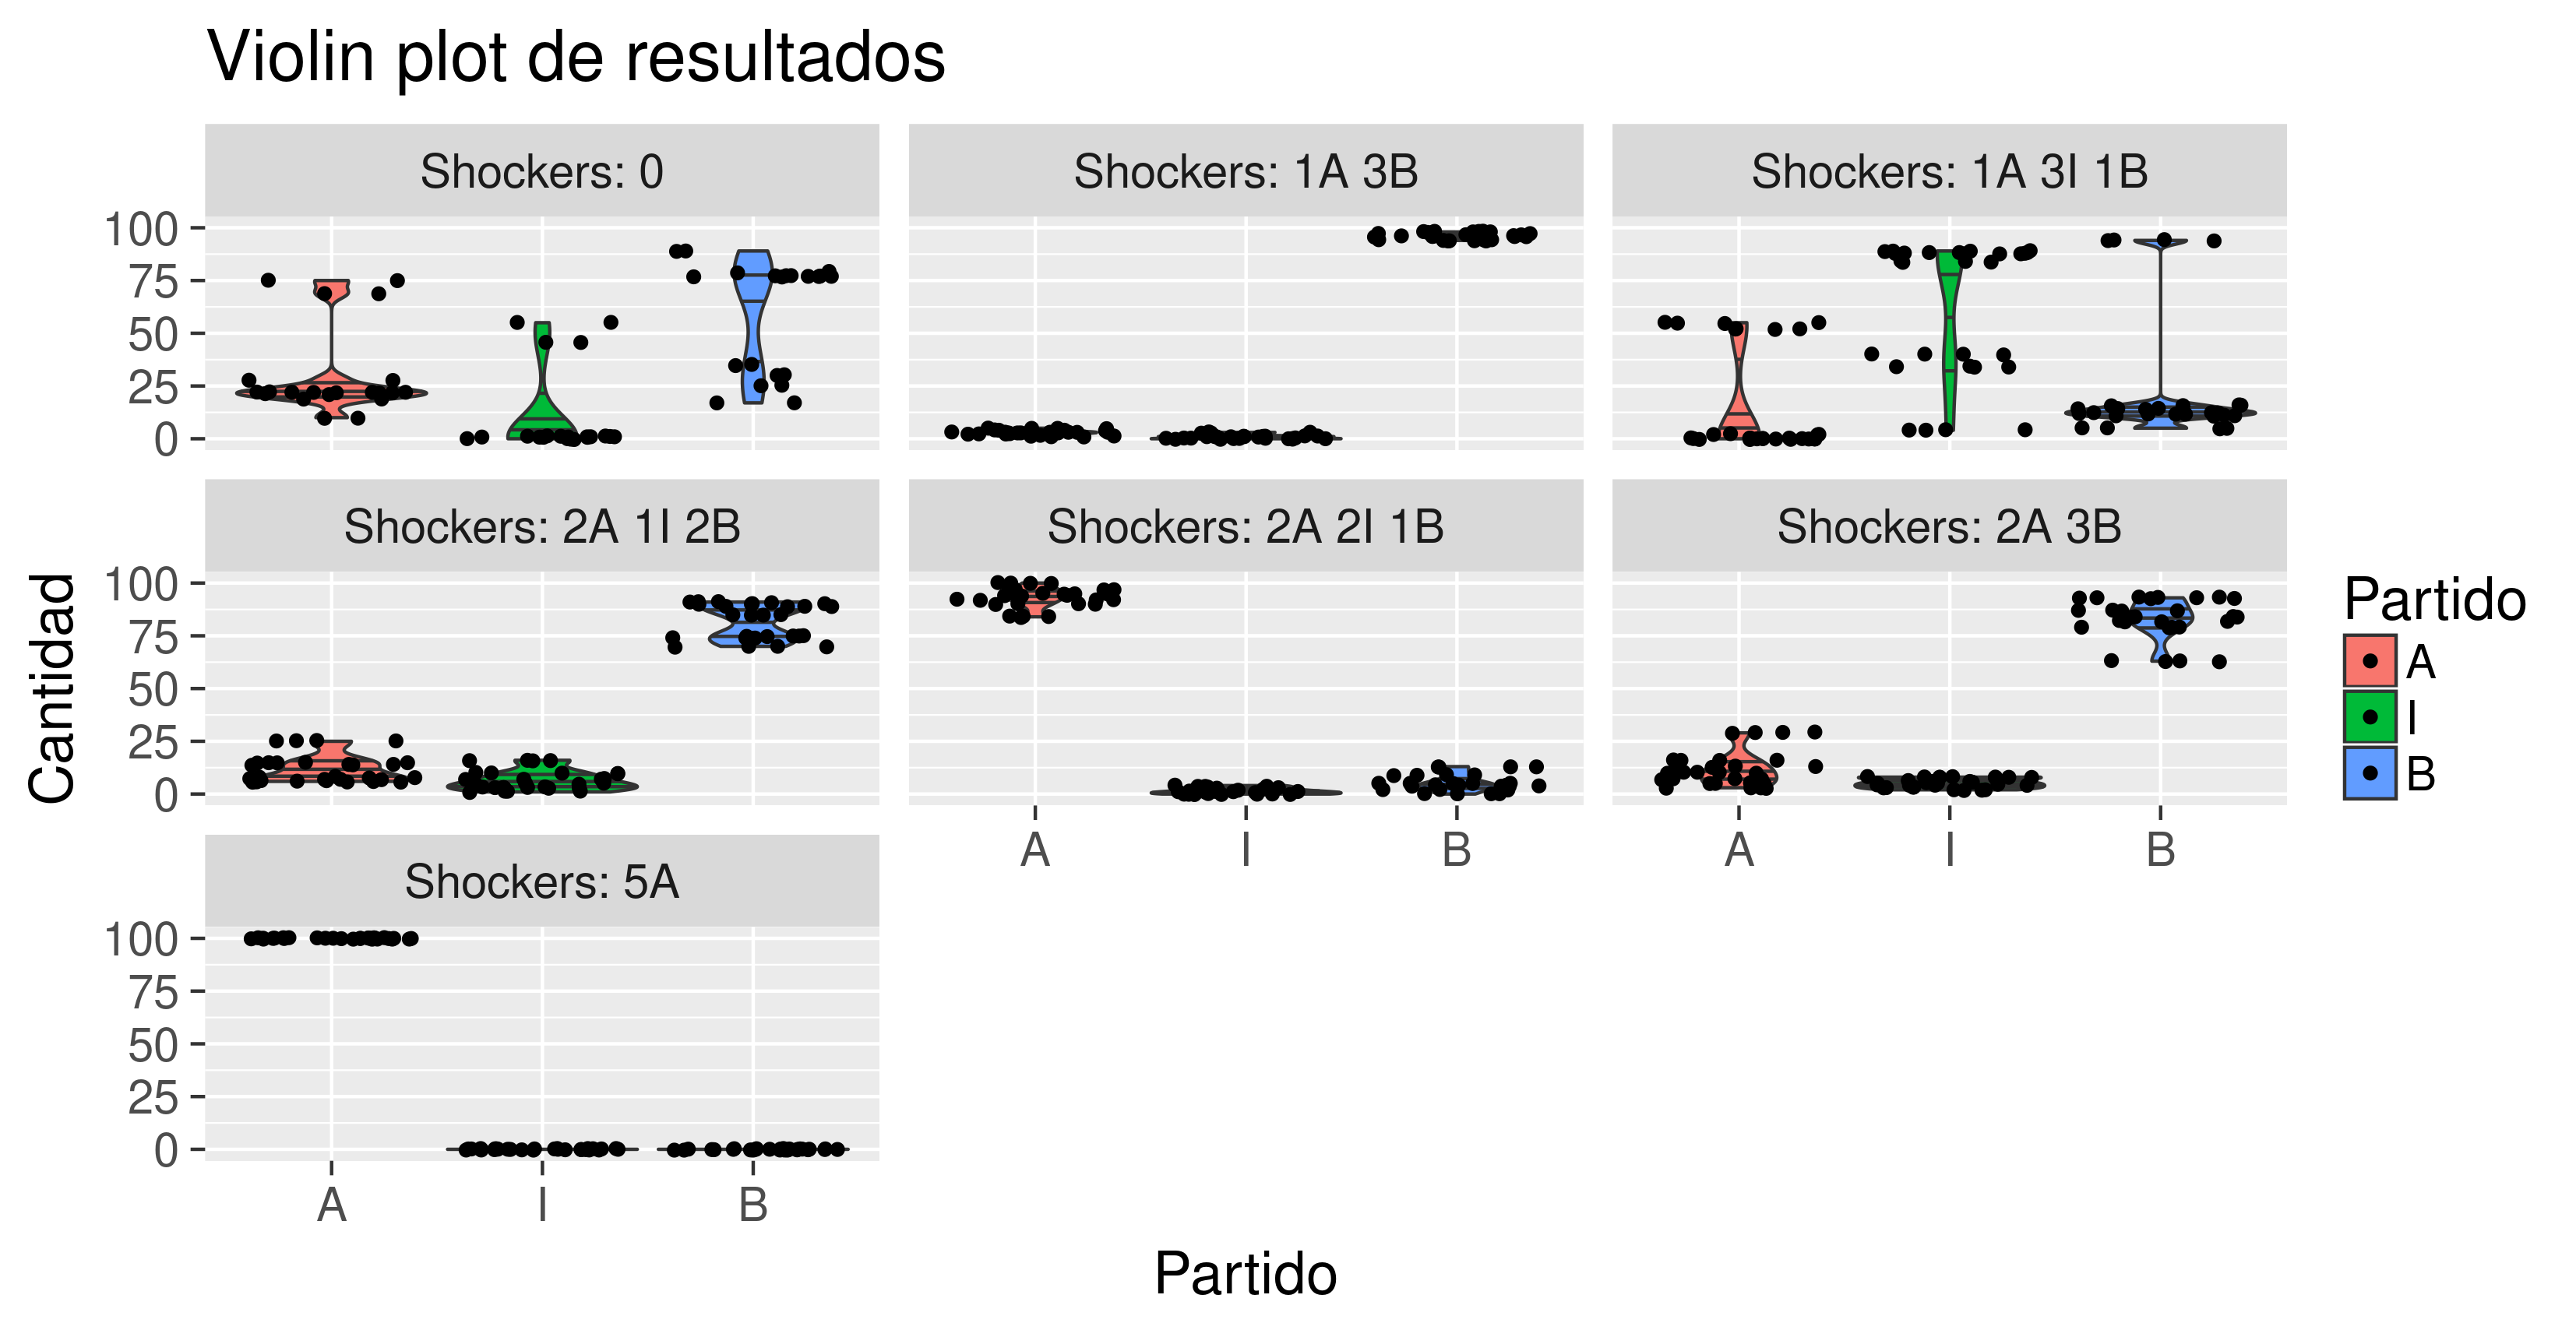
\includegraphics[scale=0.5]{imagenes/violin_resultados.png}
\caption{Vecindario de celdas utilizado para definir el comportamiento de cada agente}
\label{fig:modelo_shock_violin}
\end{figure}


